\documentclass[a4paper]{article} %format de la feuille + type de document https://en.wikibooks.org/wiki/LaTeX/Document_Structure#Document_classes
%packages nécessaire pour nos besoins
\usepackage[utf8]{inputenc}
\usepackage[T1]{fontenc}
\usepackage[english,french]{babel}
\usepackage{amsmath}
\usepackage{amssymb,amsfonts,textcomp}
\usepackage{color}
\usepackage{array}
\usepackage{hhline}
\usepackage{hyperref}
\usepackage[pdftex]{graphicx}
\usepackage{sectsty}
\usepackage{tcolorbox}
\usepackage{textcomp}
\usepackage{courier}
\usepackage[font={small,it}]{caption}
\usepackage{float}
\usepackage{graphicx}
\usepackage{caption}
\usepackage{tabularx}
\usepackage{multirow}% http://ctan.org/pkg/multirow
\usepackage{tikz}
\usepackage[top=15mm,bottom=20mm,right=50mm,left=50mm]{geometry} 
\usepackage[export]{adjustbox}


%Définition des couleurs
\definecolor{havelockBlue}{rgb}{0.004, 0.42, 0.73}
\definecolor{Monokaimagenta}{rgb}{0.86,0.08,0.24}

%utilisation de la couleur définie avant
%toutes les sections auront cette couleur
\sectionfont{\color{havelockBlue}}
%\subsectionfont{\color{havelockBlue}}
%début du document
\begin{document}

\renewcommand{\labelitemi}{$\bullet$}
\renewcommand{\labelitemii}{$\cdot$}
\renewcommand{\labelitemiii}{$\diamond$}
\renewcommand{\labelitemiv}{$\ast$}

%début d'un titre
\begin{titlepage}
            %centre les éléments
	\centering
	
	{\scshape\LARGE \color{Monokaimagenta} Laboratoire \\  \par}
	
	%espace vertical de 1 mms
	\vspace{1cm}
	
	{\Large\itshape Sven Rouvinez \& Johanna Melly\par}
	
	%http://www.personal.ceu.hu/tex/spacebox.htm
	\vfill
	Professeur\par
	%met le texte en gras 
	\textbf{Carlos Andrés Pena} \par% ajoute une ligne 
	\vspace{1cm}
	Assistant\par
	\textbf{Gaëtan Matthey}
	
	\vfill

            %affiche la date actuelle
	{\large \today\par}
	
%fin de la page de titre
\end{titlepage}

\section{Objectifs du laboratoire}
La réalisation simplifiée de la partie FETCH d'un processeur RISC\footnote{Reduced Instruction Set Computing} avec l'incrémenation du PC\footnote{Program Counter} et la lecture d'instruction ainsi qu'un mécanisme de saut et un système de gestion d'interruption.

\section{Blocs Logisim}
Nous avons décidé de séparer les blocs afin de permettre une meilleure modularité et abstraction du système FETCH.\\
\paragraph{Résumé}
\begin{itemize}
    \item     MOV\_INST détecte une instruction \textbf{MOV}
    \item     BRANCH\_INST détecte une instruction \textbf{B}
    \item     CALC\_ADR calcule le décalage lors d'une instruction \textbf{B}
    \item     FETCH\_16BITS circuit avec incrémentation du PC et lecture d'instructions
    \item     FETCH\_JUMP\_16BITS circuit avec mécanisme de saut
    \item     FETCH\_INTER\_16BITS (main) circuit avec mécanisme d'interruption
\end{itemize}
\subsection{MOV\_INST}

\begin{figure}[H]
    \centering
    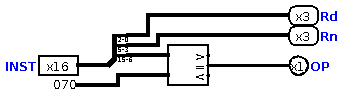
\includegraphics[width=.8\textwidth]{src/MOV_INST.png}
    \caption{Instruction MOV}
    \label{mov}
\end{figure}
\paragraph{Définition des entrées:}
\begin{itemize}
    \item     INST: code complet
    \item     0x70: code recherché
\end{itemize}

\paragraph{Définition des sorties:}
\begin{itemize}
    \item     Rd: registre destination
    \item     Rn: registre source
    \item     OP: s'active si les bits de 15 à 9 sont égal à $0001110$ (0x70)
\end{itemize}

\medskip

Ce bloc permet de détecter si une instruction \textbf{MOV} est trouvée, grâce au comparateur, dans le code de sortie de la ROM, cette instruction va charger le valeur du registre source (Rn) dans le registre destination (Rd).\\
Elle se caractérisque par le code ci-dessous : 
\\
\begin{tabular}{|ccccccc|ccc|ccc|ccc|}
    \hline
    \multicolumn{7}{|c|}{Code ARM}  & \multicolumn{3}{|c|}{Opcode} & \multicolumn{3}{|c|}{Rn} & \multicolumn{3}{|c|}{Rd}\\
    \hline
    15 & 14 & 13 & 12 & 11 & 10 & 9 & 8 & 7 & 6                    & 5 & 4 & 3                & 2 & 1 & 0 \\
    \hline
    0  & 0  & 0  & 1  & 1  & 1  & 0 & 0 & 0 & 0                    & 1 & 0 & 0                & 1 & 0 & 1 \\
    \hline     
    \end{tabular}
\\
\begin{itemize}
    \item     Code ARM : instruction ARM à effectuer
    \item     Opcode : instruction à effectuer par l'ALU
    \item     Rn : registre source
    \item     Rd : registre destination
\end{itemize}


\subsection{BRANCH\_INST} \label{branchinst}
\begin{figure}[H]
    \centering
    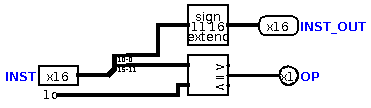
\includegraphics[width=.8\textwidth]{src/BRANCH_INST.png}
    \caption{Instruction BRANCH}
    \label{branch}
\end{figure}

\paragraph{Définition des entrées:}
\begin{itemize}
    \item     INST: code complet
    \item     0x1c: code recherché
\end{itemize}

\paragraph{Définition des sorties:}
\begin{itemize}
    \item     INST\_OUT: contient l'adresse de retour
    \item     Rn: registre source
    \item     OP: s'active si les bits de 15 à 11 sont égal à $00011$ (0x70)
\end{itemize}

\medskip
Grâce à ce bloc, le système sera capable d'effectuer un saut inconditionnel. Pour calculer l'adresse de retour, il faut effectuer une opération: $PC + Adresse*2 + 4$ (voir \ref{bl_calc_adr}).\\

\begin{tabular}{|ccccc|ccccccccccc|}
    \hline
    \multicolumn{5}{|c|}{Code ARM}  & \multicolumn{11}{|c|}{Offset}\\
    \hline
    15 & 14 & 13 & 12 & 11          & 10 & 9 & 8 & 7 & 6 & 5 & 4 & 3 & 2 & 1 & 0 \\
    \hline
    1  & 1  & 1  & 0  & 0           & 1  & 0 & 0 & 0 & 0 & 0 & 0 & 0 & 0 & 0 & 0\\
    \hline     
    \end{tabular}
    \\
\begin{itemize}
    \item     Code ARM : instruction ARM à effectuer
    \item     Offset: adresse relative par rapport au PC
\end{itemize}


\paragraph{Exemple:} dans notre cas, nous avons \textit{B ADR\_SAUT\_1} dans notre fichier d'instructions ce qui équivaut à 0xe7fc. Donc si nous prenons le tableau du haut et que nous faisons la conversion en binaire:
\\
\begin{tabular}{|ccccc|ccccccccccc|}
    \hline
    \multicolumn{5}{|c|}{Code ARM}  & \multicolumn{11}{|c|}{Offset}\\
    \hline
    15 & 14 & 13 & 12 & 11          & 10 & 9 & 8 & 7 & 6 & 5 & 4 & 3 & 2 & 1 & 0 \\
    \hline
    1  & 1  & 1  & 0  & 0           & 1  & 1 & 1 & 1 & 1 & 1 & 1 & 1 & 1 & 0 & 0\\
    \hline     
    \end{tabular}
    
    \medskip
Seul les bits 10 à 0 nous intéressent pour le calcul, c'est pourquoi il y a un bit extender de 11 bits $\rightarrow$ 16 bits pour travailler sur la même base.\\
Ensuite, nous effectuons le calcul avec un PC à $4$ et un INST\_OUT de 0xfffc: $4 + 1111111111111100 * 2 + 4=0000$ donc l'adresse de retour sera $0000$

\subsection{CALC\_ADR} \label{bl_calc_adr}
\begin{figure}[H]
    \centering
    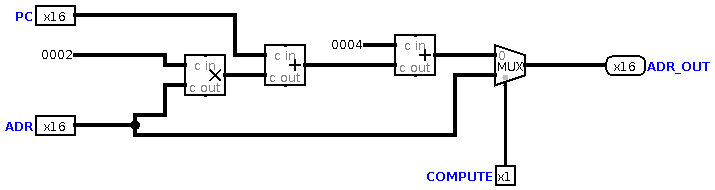
\includegraphics[width=.8\textwidth]{src/CALC_ADR.png}
    \caption{Calcul du saut}
    \label{bl_calc_adr}
\end{figure}
\paragraph{Définition des entrées:}
\begin{itemize}
    \item     PC: program counter
    \item     ADR: adresse à décaler
    \item     0x0002: multiplication par 2
    \item     0x0004: addition de 4
\end{itemize}

\paragraph{Définition des sorties:}
\begin{itemize}
    \item ADR\_OUT: contient l'adresse du saut
    \item COMPUTE: si à $1$ le calcul de l'adresse du saut ne sera pas effectué
\end{itemize}
\medskip
Dans ce bloc, l'adresse fournie va subir 3 opérations. Elle va être multipliée par 2 (offset), addionnée au PC, puis additionnée à 4.\\
L'entrée \textbf{COMPUTE} permet de passer outre ce calcul si l'instruction venait à être différente à un MOV.
\\
Si, par exemple, l'entrée \textbf{ADR} 0xfffc, et le \textbf{PC} 0x0004 (cas que nous rencontrons plus tard dans ce labo) en multipliant par 2 on obtient 0xfff8, puis en ajoutant l'entrée PC à 0x0004 on obient 0xfffc, et, pour finir, en ajoutant 4, on obtient 0x20000. Ainsi, puisque la sortie est sur 4 bits, on obtient 0x0000 en \textbf{ADR\_OUT}. On sait donc que l'adresse après saut est 0x0000.

\subsection{FETCH\_16BITS}
\begin{figure}[H]
    \centering
    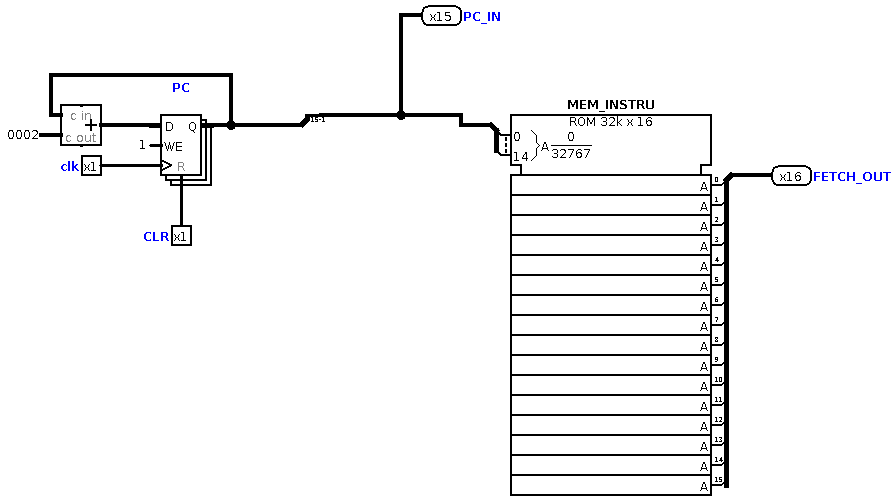
\includegraphics[width=1\textwidth]{src/FETCH.png}
    \caption{Fetch 16 bits}
    \label{fetch_16bits}
\end{figure}
\paragraph{Définition des entrées:}
\begin{itemize}
    \item     PC: program counter
    \item     clk: horloge
    \item     CLR: reset
\end{itemize}

\paragraph{Définition des sorties:}
\begin{itemize}
    \item FETCH\_OUT: instruction en sortie
    \item     PC\_IN: adresse en sortie du splitter
\end{itemize}
\medskip
<<<<<<< HEAD
Ce circuit permet de parcourir les adresses en mémoire. On a un register 16 bits qui parcourt les adresses. Comme on veut ignorer la première adresse (0), un splitter à la sortie du registre va prendre 15 bits uniquement, et le bit de poids faible ne va pas être retenu. La raison de la suppression du bit de poids faible, est que les adresses sont par bloc de 2 bytes, et auront donc toujours un nombre pair. Ainsi, le bit de poids faible n'est pas signification puisqu'il sera toujours à 0. Puisqu'on veut parcourir toutes les adresses, et qu'en supprimant le bit de poids faible de l'adresse on divise l'adresse par deux, on ajoute un additionneur +2 au début du regiter. Cela va permettre de doubler l'adresse, et ainsi, en supprimant de bit de poids faible, on obtient l'adresse attendue. Ainsi, grâce à cet addtionneur, on sélectionne une nouvelle adresse à chaque coup d'horloge.
=======
Ce circuit permet de parcourir les adresses en mémoire. \\
Il y a un register 16 bits qui parcourt les adresses. Pour ignorer le premier bit (0), un splitter à la sortie du registre va prendre 15 bits uniquement (1..15), et le bit de poids faible ne va pas être retenu. Mais puisqu'il faut parcourir toutes les adresses, et qu'en supprimant le bit de poids faible de l'adresse elle est divisée par deux, on ajoute un additionneur +2 au début du register. Cela va permettre de doubler l'adresse, et ainsi, en supprimant de bit de poids faible, on obtient l'adresse attendue. Ainsi, grâce à cet addtionneur, on sélectionne une nouvelle adresse à chaque coup d'horloge.
>>>>>>> 2d10c84d805f7b661152fd7edecbd143e27f54c3
\subsection{FETCH\_JUMP\_16BITS}
\begin{figure}[H]
    \centering
    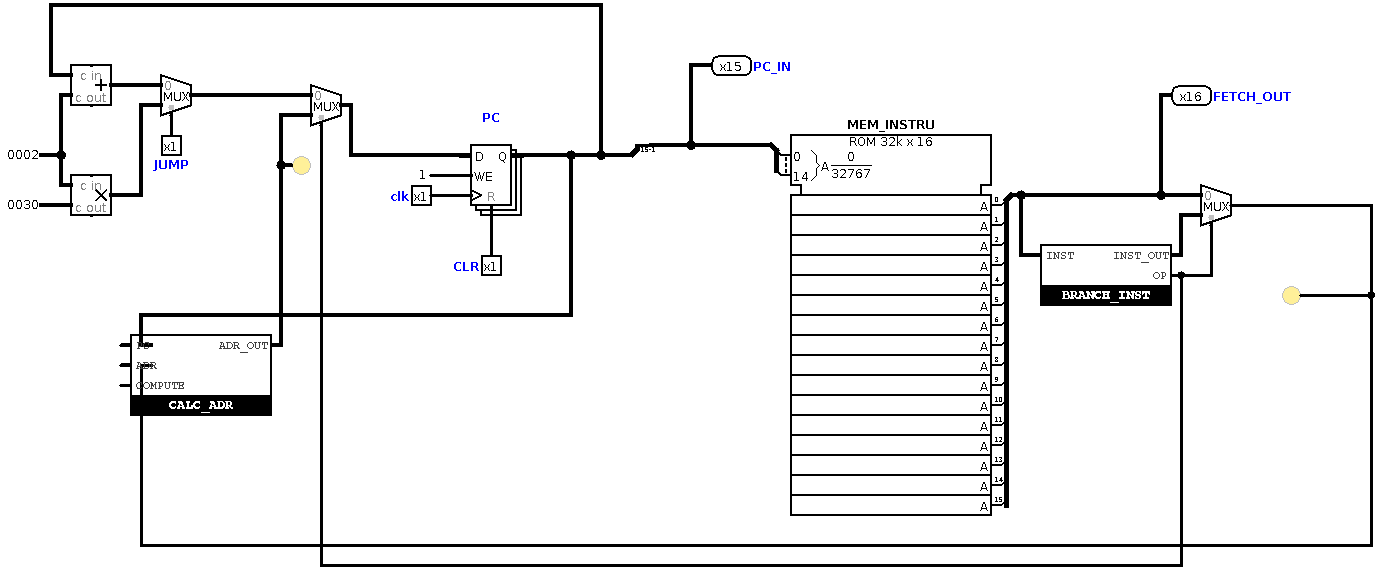
\includegraphics[width=1\textwidth]{src/FETCH_JUMP.png}
    \caption{Mécanisme de saut}
    \label{fetch_jump}
\end{figure}
Le registre PC contient l'adresse actuelle. Un multiplexer placé avant va être à zéro tant que l'instruction 0xe7fc n'est pas rencontrée. Si elle est rencontrée, alors le bloc BRANCH\_INST (voir \ref{branchinst}) va renvoyer 1 à sa sortie \textbf{OP}, car les bits 15 à 11 de l'instruction 0xe7fc correspondent à 0x1c (instruction de saut), qui est précisément ce qui est recherché dans le bloc BRANCH\_INST. Ainsi, comme il renvoie un 1, c'est maintenant la sortie du bloc CALC\_ADR qui va être prise en compte par le multiplexers mentionné plus haut. \\
Ce bloc CALC\_ADR prend en entrée \textbf{ADR} la sortie \textbf{INST\_OUT} du bloc BRANCH\_OUT, qui se trouve être, en héxadécimal, les bits 10 à 0 de l'instruction 0xe7fc, qui correspondent à 0xfffc, et entrée \textbf{PC} 0x0004. Dans le bloc CALC\_ADR, 0xfffc subit la suite d'opérations mentionnées dans la description de ce bloc (voir \ref{bl_calc_adr}), pour calculer l'adresse de saut, et donc la sortie sera 0x0000. Donc, à chaque fois qu'on va atteindre l'instruction 0xe7fc, on va sauter à l'adresse 0x0000.
\\
Dans ce circuit, il faut pouvoir effectuer un saut à l'adresse 0x0018, en enclenchant un bouton \textbf{JUMP}. 
\\Pour ce faire, un multiplexer a été ajouté pour choisir entre l'adresse du PC (toujours additionnée à 2, pour permettre une adresse correcte lors du retrait du bit de poids faible (comme expliqué dans le bloc FETCH\_16BITS), ou l'adresse 0x0030. Ainsi, lorsqu'on fait passer le multiplexer à 1 (grâce au pin \textbf{JUMP}, c'est l'adresse 0x0030 qui va être utilisée. Comme on retire toujours le bit de poids faible, cette adresse se retrouve divisée par 2 et on obtient bien 0x0018.
\pagebreak

\subsection{FETCH\_INTER\_16BITS}

\begin{figure}[H]
    \centering
    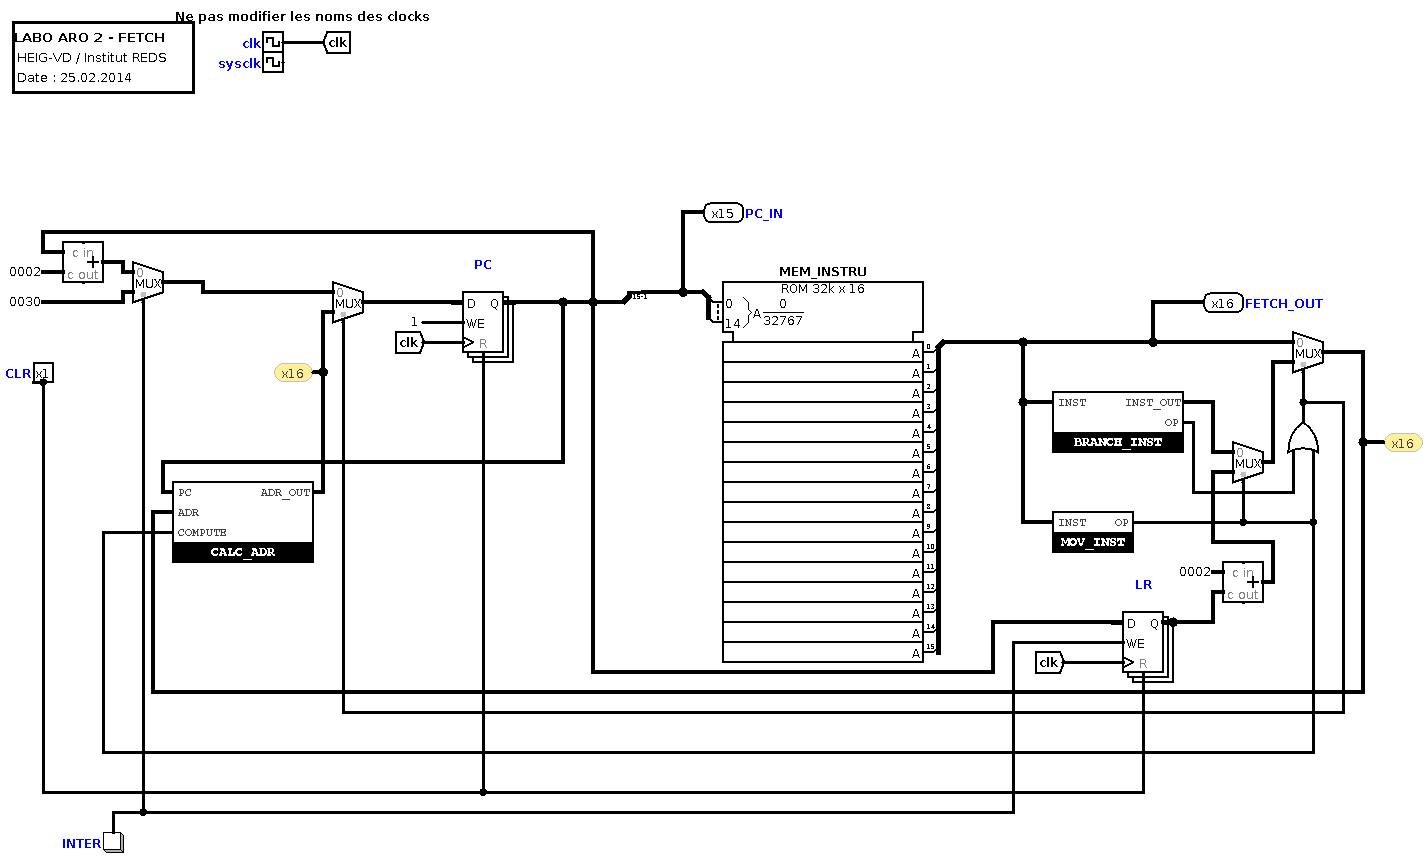
\includegraphics[width=1\textwidth]{src/FETCH_INTER.png}
    \caption{Mécanisme d'interruption}
    \label{fetch_inter}
\end{figure}

\paragraph{Définition des entrées:}
\begin{itemize}
    \item     PC: program counter
    \item     CLR: reset
\end{itemize}

\paragraph{Définition des sorties:}
\begin{itemize}
    \item FETCH\_OUT: instruction en sortie
    \item PC\_IN: adresse en sortie du compteur, après le retrait du bit de poids faible
    \item Rd: registre destination
    \item Rn: Registre source
\end{itemize}
\medskip
Ce bloc regroupe tous les blocs précédent, et permet de simuler une interruption. Les conditions de ce blocs étaient les suivantes:
\begin{itemize}
   \item Quand on presse le bouton INTER, la valeur suivante du PC est chargée dans LR\footnote{Link Register}
   \item À ce moment, le PC est chargé avec l'adresse 0x30
   \item L'intruction 1c2c doit être détectée et la valeur du registre 5 (LR) doit être chargée dans le 4 (PC) (MOV r4, r5)
\end{itemize}
\medskip
Une grande partie de ce circuit fonctionne comme le précédent, à savoir: un MUX permet de choisir entre l'adresse à laquelle est additionnée 2 à chaque coup d'horloge, ou l'adresse 0x30, qu'on veut atteindre lorsque l'on presse le bouton \textbf{INTER}. On a ensuite ensuite un registre 16 bits, dont on ignore le dernier bit en sortie. Grâce au +2 en amont, l'adresse est correcte lorsqu'elle est transmise à la mémoire. On peut facilement le vérifier grâce à la sortie \textbf{PC\_IN}. Ensuite, nous retrouvons inévitablement la mémoire, dont l'instruction de sortie est déterminée par l'adresse \textbf{PC\_IN} en entrée de celle-ci.\medskip

<<<<<<< HEAD
La partie suivante diffère légèrement. Il y a tout d'abord le bloc \text{BRANCH\_INST} qui permet de détecter les inctructions de saut. Ainsi, l'instruction 0xe7fa en mémoire est atteinte (à l'adresse 0x0004), les bits 15 à 11 de l'instruction équivalent à 0b11100. Additionnés à 0x1c dans \textbf{BRANCH\_INST}, il y a bien un bit d'overflow, et l'instruction JUMP va donc être délenchée. En sortie op, il y aura, comme expliqué dans le bloc \textbf{BRANCH\_INST} (voir ref \ref{branchinst}), les bits 10-0 de 0xe7fa, donc 0xfffa. Ces bits sont en entrée dans le bloc \textbf{CALC\_ADR}, qui va, comme expliqué précédemment, effectuer les diverses opérations qui permettent de caculer l'adresse de saut. Cette adresse sera égale à 0x0000, ainsi à chaque fois que l'instruction 0xe7fa est effectuée, un saut à l'adresse 0x0000 de la mémoire est effectué.\\
L'interupteur \textbf{INTER}, lorsqu'il est pressé, permet de choisir l'adresse 0x30 et donc de faire un saut à l'adresse 0x30 dans la mémoire. L'INTER est aussi relié au registre LR. Ainsi, lorsque INTER est activé, l'adresse PC est chargée dans le LR, juste avant qu'il passe à 0x30.\medskip \\
=======
La partie suivante diffère légèrement. On retrouve d'abord le bloc \text{BRANCH\_INST} qui permet de détecter les inctructions de saut. Ainsi, lorsque l'on atteint l'instruction 0xe7fa en mémoire (à l'adresse 0x0004), les bits 15 à 11 de l'instruction équivalent à 0b11100. Additionné à 0x1c dans \textbf{BRANCH\_INST}, on a bien un bit d'overflow et donc l'instruction de saut va être délenchée. En sortie \textbf{OP}, on aura, comme expliqué dans le bloc \textbf{BRANCH\_INST} (voir \ref{branchinst}), les bits 10-0 de 0xe7fa, donc 0xfffa. Ces bits sont en entrée dans le bloc \textbf{CALC\_ADR}, qui va, comme expliqué précédemment, effectuer les diverses opérations qui permettent de caculer l'adresse de saut. Cette adresse sera égale à 0x0000, ainsi à chaque fois que l'instruction 0xe7fa est effectuée, on retrourne à l'adresse 0x0000 de la mémoire.\\
L'interrupteur \textbf{INTER}, lorsqu'il est pressé, permet de choisir l'adresse 0x30 et donc de faire un saut à l'adresse 0x30 dans la mémoire. L'INTER est aussi relié au registre LR. Ainsi, lorsque INTER est activé, l'adresse suivante du PC est chargée dans le LR, juste avant qu'il passe à 0x30.\medskip \\
>>>>>>> 2d10c84d805f7b661152fd7edecbd143e27f54c3

Le bloc \textbf{MOV\_INST} permet de détecter l'instruction MOV. Il va détecter si les bits 15 à 6 sont égal à 0x70 (MOV). Ici, l'instruction à détecter est 0x1c2c. Les bits 15-6 de cette instruction sont 0b0001110000, ce qui correspond bien à 0x70. 
\\Ainsi, l'instruction MOV va être activée. Le registre source (ici r5) correspond aux bits 5-3 et le registre destination (ici r4) correspond aux bits 2-0. On peut voir sur la figure ci-dessous la détection de l'instruction MOV, et les registres source et destination en sortie de \textbf{MOV\_INST}

\begin{figure}[H]
    \centering
    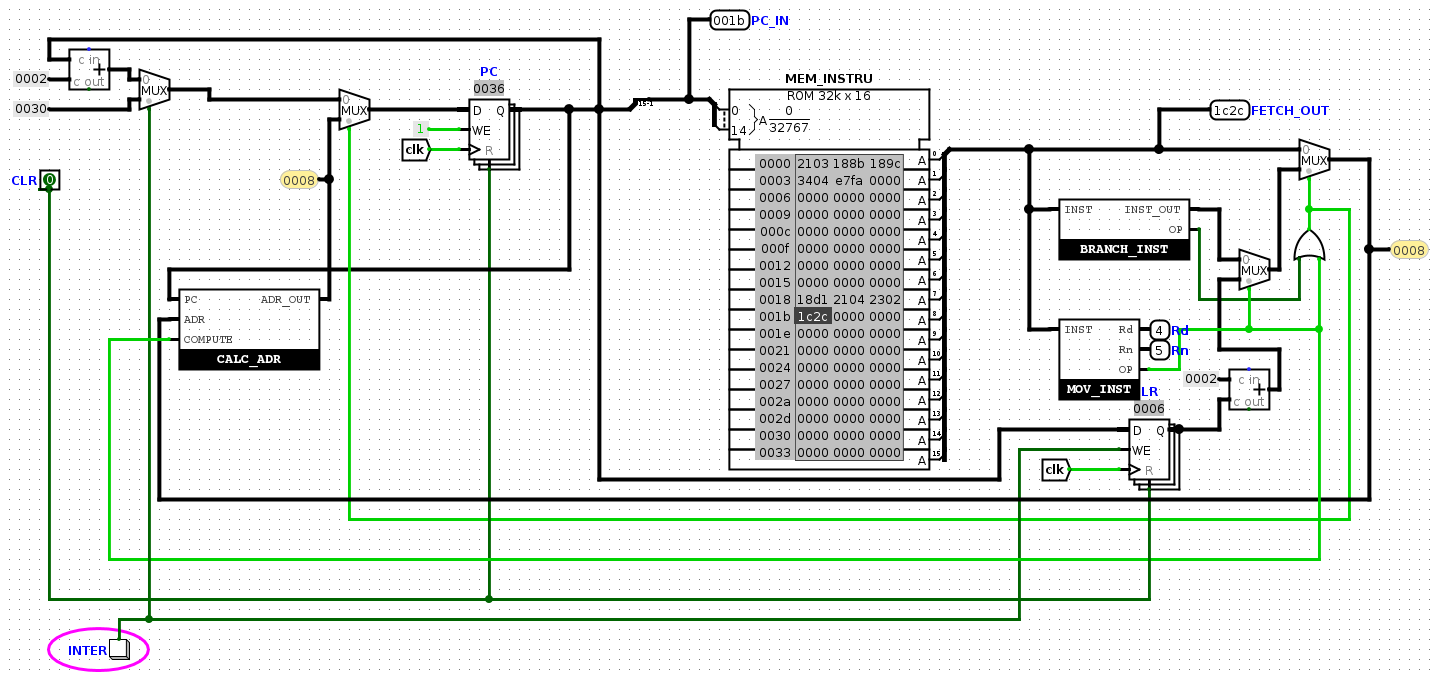
\includegraphics[width=1\textwidth]{src/FETCH_INTER_1c2c.png}
    \caption{Intruction MOV}
    \label{fetch_inter}
\end{figure}

\section{Conclusion}
Dans ce laboratoire, nous avons pu mettre en pratique la théorie vue en classe, qui peut parfois être un peu floue jusqu'à avoir un exemple concret. Nous avons appris à manipuler des adresses de mémoire et des instructions, compris le fonctionnement de ces dernières et la façon dont elles étaient segmentées, chaque portion de bits contenant une information qui permet d'effectuer les bonnes opérations aux bons endroits. \\
L'utilisation de blocs permet d'ajouter une couche d'abstraction et donc de modularité lorsque la connexion de différents circuits (comme dans le main) est nécessaire.
\section{Annexes}

\end{document}